\documentclass[11pt,a4paper]{report}
\usepackage[utf8]{inputenc}
\usepackage{amsmath}
\usepackage{amsfonts}
\usepackage{amssymb}
\usepackage{graphicx}
\usepackage{enumitem}
\usepackage[left=2cm, right=2cm, top=4.5cm, bottom=2cm]{geometry}

\begin{document}
	%Portada
	\begin{titlepage}
		\centering
		{\scshape\LARGE Universidad Nacional Autónoma de México \par}
		\vspace{1cm}
		{\scshape\Large Probabilidad I\par}
		\vspace{1.5cm}
		{\huge\bfseries Tarea Examen\par}
		\vspace{.5cm}

		{\Large\itshape Alan Ernesto Arteaga Vázquez \par}
		 \vspace{.5cm}
		{\Large\itshape Raúl Llamosas Alvarado \par}
		 \vspace{.5cm}
		{\Large\itshape Edgar Quiroz Castañeda \par}
	    \vspace{.5cm}
		{\Large\itshape Jean Paul Ruiz Melo\par}
		\vspace{.5cm}
		{\Large\itshape Sandra Del Mar Soto Corderi \par}

		\vfill
		 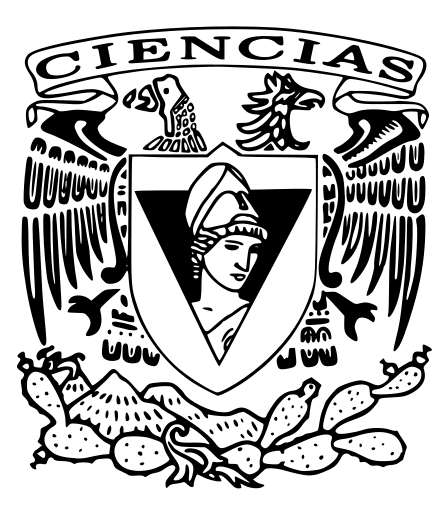
\includegraphics[width=0.3\textwidth]{escudo.png}
		\vfill

		{\large Lunes 3 de Diciembre del 2018 \par}
	\end{titlepage}

	\pagebreak
	\setlength{\voffset}{-0.75in}
	\setlength{\headsep}{5pt}

	%Ejericios
	\begin{enumerate}
		%1
		\item{
		
		Considere el experimento de lanzar dos tetraedros cuyos lados están numerados del 1 al 4. Sean $Y_{1},Y_{2}$ los números más pequeño y más grande obtenidos en las caras superiores respectivamente. 
		    
		    \begin{enumerate}
		        %(a)
		        \item {Encuentre la función de densidad conjunta de $Y_{1},Y_{2}$}
		        %(b)
		        \item{Obtenga la densidad condicional de $Y_{2}$ dado $Y_{1}$ para cada uno de los posibles valores de $Y_{1}$}
		        %(c)
		        \item{Encuentre $E(Y_{1}Y_{2}),E(Y_{1}),E(Y_{2})$}
		        %(d)
		        \item{¿Son $Y_{1} $ y $Y_{2}$ independientes?}
		    \end{enumerate}
            
		}

		%2
		\item{
		Suponga que X es una variable aleatoria con distribución $Bin(100,\frac{1}{5})$. Utilizando el teoerema de DeMoivre-Laplace, calcular $P(15\leq X \leq 25)$. 
		
		}

		%3
		\item{
            En una tarde soleada, Augusto lanza dos dados 2160 veces (él casi no tiene nada que hacer). Sea X el número de veces que 2 aparece en alguna de las caras. Encontrar la probabilidad de que X sea menor a 55.
		}

		%4
		\item{
			Sean $X_{1},...,X_{n}$ variables aleatorias independientes. Use la función generadora de momentos para encontrar la distribución de $\sum_{i=1}^{n}X_{i}$ en los siguientes casos:\\
			\begin{enumerate}
			    %(a)
			    \item {Si $\forall i \ \in \lbrace 1,..,n \rbrace \ X_{i} \sim Gamma(r,\lambda)$}
			    
			    %(b)
			    \item{Si $\forall i \ \in \lbrace 1,..,n \rbrace \ X_{i} \sim Gamma(r_{i},\lambda)$ }
			    %(c)
                \item{Si $\forall i \ \in \lbrace 1,..,n \rbrace \ X_{i} \sim exp(\lambda)$ }
                %(d)
                \item{Si $\forall i \ \in \lbrace 1,..,n \rbrace \ X_{i} \sim Geo(p)$ }
                %(e)
                \item{Si $\forall i \ \in \lbrace 1,..,n \rbrace \ X_{i} \sim BinNeg(r,p)$ }
                %(f)
                \item{Si $\forall i \ \in \lbrace 1,..,n \rbrace \ X_{i} \sim BinNeg(r_{i},p)$ }
                %(g)
                \item{Si $\forall i \ \in \lbrace 1,..,n \rbrace \ X_{i} \sim Poisson(\lambda)$ }
                %(h)
                \item{Si $\forall i \ \in \lbrace 1,..,n \rbrace \ X_{i} \sim Bin(n,p)$ }
                %(i)
                \item{Si $\forall i \ \in \lbrace 1,..,n \rbrace \ X_{i} \sim Bin(n_{i},p)$ }
                %(j)
                \item{Si $\forall i \ \in \lbrace 1,..,n \rbrace \ X_{i} \sim N(\mu,\sigma_{i}^2)$ }
			\end{enumerate}
		}

		%5 
		\item{
		Sea $S_{n}$ el número de éxitos en n ensayos Bernouilli independientes. Demuestre que $$P(|\frac{S_{n}}{n}-p|\geq \epsilon)\leq \frac{1}{4n\epsilon^2}$$
			
		}

		%6
		\item{
		Sea S el número de águilas en 1,000,000 lanzamientos de una moneda honesta. Use (a) la desigualdad de Chebyshev y (b) el Teorema del Límite Central para estimar la probabilidad de que S esté entre 499,500 y 500,500.
		}

		%7
		\item{
			
          Si $X \sim Gamma(n,1)$ aproximadamente que tan grande debe ser n para que 
          $$P[|\frac{X}{n}-1| > 0.01] < 0.01$$
          
          Definamos $X_{i} \sim Exp(1)$, como hemos visto en clase, Gamma es una generalización de Exponencial, entonces podemos decir que:
          
          $X = \sum_{i=1}^{n} X_{i}$,
          
          Así podemos ver que:
          
           $P[|\frac{X}{n}-1| > 0.01] < 0.01 = P[|\frac{\sum_{i=1}^{n} X_{i}}{n}-1| > 0.01] < 0.01$\\
           
           $= P[|\frac{\sum_{i=1}^{n} X_{i} -n}{n}| > 0.01] < 0.01$\\
           
           Sabemos que el Teorema del Limite Central dice que:
				
 				z = $\frac{\sum_{i=1}^{n} X_{i} - \mu n }{\sigma \sqrt{n}}  \xrightarrow{n \to \infty}  z \sim N(0,1)$\\
			            
          Vemos que la exponencial y varianza valen 1, es decir, $\mu = 1$ y $\sigma = 1$, así que para que nuestra expresión sea igual al teorema del límite central, necesitamos una $\sqrt{n}$ en el denominador, esto lo podemos conseguir multiplicando por $\sqrt{n}$ los dos lados de la desigualdad, esto no afecta, ya que la raíz cuadrada respeta el valor absoluto, entonces tenemos:
          
          $= P[|\frac{\sum_{i=1}^{n} X_{i} -n}{\sqrt{n}}| > 0.01\sqrt{n}] < 0.01$
          
          Vemos que es igual a la definición del Teorema del Límite Central y aplicandolo tenemos que cuando $n \to \infty$:
          
          $P( |z| > 0.01\sqrt{n} ) < 0.01$
          
          $ = (1 - P(z \leq 0.01\sqrt{n})) < 0.01$
          
          $ = (1 - \phi(0.01\sqrt{n})) < 0.01$
          
          $ = - \phi(0.01\sqrt{n}) < 0.01 - 1$
          
         $ = \phi(0.01\sqrt{n}) > 0.99$
          
        Revisando la tabla de distribución de la normal, podemos observar que el primer valor donde $\phi$ es mayor a 0.99 es 2.33, entonces:
        
        $\phi(2.33) > 0.99$  y  $\phi(0.01\sqrt{n}) > 0.99$\\
        
        De ahí, 
        
        $0.01\sqrt{n} = 2.33$
        
        $\sqrt{n} = \frac{2.33}{0.01}$
        
        $n = (\frac{2.33}{0.01}) ^ 2 = 54289$\\
        
        Por lo tanto n debe ser al menos 54289 para que $P[|\frac{X}{n}-1| > 0.01] < 0.01$\\
		}

		%8
		\item{
			Sean $X_{1},...,X_{20}$ variables aleatorias independientes tales que $\forall i \ \in \lbrace 1,...,20 \rbrace \ X_{i} \sim Poisson(\lambda) $ con media 1.\\
			\begin{enumerate}
			    %(a)
			    \item{Utilice la desigualdad de Markov para obtener una cota para $P[\sum_{i=1}^{20}X_{i}>15]$} 
			    
			    Sabemos que la desigualdad de Markov dice que:
			    
			    $P(g(x) \geq k) \leq \frac{E(g(x))}{k}$\\
			    
			    Ya que la esperanza de cada $X_{i}$ es 1, la esperanza de la suma, es 20.
		    
			    Sustituimos en la desigualdad y tenemos que:\\
			    
			    $P(\sum_{i=1}^{20}X_{i}>15) < \frac{E(\sum_{i=1}^{20}X_{i})}{15} = \frac{20}{15}$\\
			    
			    Otra forma de ver el problema es:
			    
			    $P(\sum_{i=1}^{20}X_{i}\geq 16) \leq \frac{E(\sum_{i=1}^{20}X_{i})}{16} = \frac{20}{16}$\\
			        
			    
			    %(b)
			    \item{Utilice el Teorema del Limite Central para aproximar $P[\sum_{i=1}^{20}X_{i}>15]$}
			    
				Sabemos que el Teorema del Limite Central dice que:
				
 				z = $\frac{\sum_{i=1}^{n} X_{i} - \mu n }{\sigma \sqrt{n}}  \xrightarrow{n \to \infty}  z \sim N(0,1)$\\
			    
				Ya que la esperanza de la suma es 20, al ser distribución poisson, sabemos que la varianza es igual a la esperanza, entonces la esperanza de la suma también es 20, es decir $\mu = 20$ y $\sigma = \sqrt{20}$, sustituimos en el teorema y tenemos:
				
				z = $\frac{\sum_{i=1}^{20} X_{i} - 20n }{\sqrt{20n}}  \xrightarrow{n \to \infty}  z \sim N(0,1)$\\
				
				Entonces tenemos que:
				
				$P(z > \frac{15 - 20}{\sqrt{20}}) = 1 - P(z \leq \frac{15 - 20}{\sqrt{20}}) = 1 - \phi (\frac{15 - 20}{\sqrt{20}}) = 1 - \phi(-\frac{\sqrt{5}}{2})$
				$= 1 - (1 - \phi (\frac{\sqrt{5}}{2})) = \phi(\frac{\sqrt{5}}{2})$
				$\approx \phi(1.11) = 0.8665$\\
				
				Por lo tanto:
				
				$P[\sum_{i=1}^{20}X_{i}>15] \approx 0.8665$\\
			\end{enumerate}
		}

		%9
		\item{
	    Sea $\lbrace X_{i} \rbrace _{i=1}^{\infty}$ una sucesión de variables aleatorias independientes. Suponga que $E(X_{i})=0$ y $Var(X_{i})=\sigma_{i}^{2}$ y suponga también que:
	            $$\lim_{n \rightarrow \infty}\sum_{i=1}^{n}\frac{\sigma_{i}^{2}}{n^2}=0$$
	   Demuestre que para cualquier $\epsilon >0$
	                $$P(\frac{|\sum_{i=1}^{n}X_{i}|}{n}>\epsilon)\rightarrow 0$$
	   Cuando $n\rightarrow \infty$.\\
	   Use lo anterior para probar que si $\lbrace Y_{i} \rbrace_{i=1}^{\infty}$ son variables aleatorias independientes tales que $Y_{i}\sim Bnnlli(p_{i})$ entonces para cualquier $\epsilon>0$, 
	                $$P(|\frac{\sum_{i=1}^{n}Y_{i}}{n}-p(n)|\leq \epsilon)\rightarrow 1$$
	   Cuando $n\rightarrow \infty$ donde $p(n)=\frac{\sum_{i=1}^{n}p_{i}}{n}$
		}

		%10
		\item{
			Explique por qué una variable aleatoria con distribución $Gamma(r,\lambda)$ tiene aproximadamente una distribución normal cuando r es grande. 
		}

		
	\end{enumerate}
\end{document}
